\documentclass[a4j, 11pt]{jsarticle}

\usepackage{graphicx}
\usepackage[dvipdfmx]{color}
\usepackage{bm}
\usepackage{amsmath}
\usepackage{amssymb}
\usepackage{amsthm} 
\usepackage{url}
\usepackage{here}
\usepackage{tcolorbox}
\usepackage{otf}
\usepackage{xhfill}
\usepackage{ulem}
\parindent = 0pt
\tcbuselibrary{breakable, skins, theorems}

\numberwithin{equation}{section}
\renewcommand{\proofname}{\textbf{証明}}
\renewcommand{\labelitemii}{・}
\renewcommand{\theenumi}{\ajLabel\ajMaru{enumi}}
\newtheorem{theorem1}{定理}[section]

\DeclareMathOperator*{\argmin}{argmin}
\DeclareMathOperator*{\argmax}{argmax}

\title{Attention機構とTransformer} 
\author{長谷川駿一}
\date{2023年5月26日 }
\begin{document}
\maketitle
\section{はじめに}
 \textbf{Transformer}とは,2017年にGoogleから発表した論文「Attention Is All You Need」\cite{all}で提案され,自然言語処理の分野において大きな貢献をもたらしたDNNベースのモデルである.自然言語処理分野で有名なモデルであるBERTやGPTなどにも使用されており,今日では,音声分野や画像による物体検出など,さまざまな分野で応用されている.\\
 本稿では,Transformerの構造から,なぜTransformerがここまで躍進したのかを説明し,実装してみた結果を発表する.\\

\section{Transformer以前の提案手法}
\subsection{Seq2Seq}
 Transformerを含む自然言語処理モデルの多くは\textbf{Encoder-Decoder}モデルで構成される.\\
 Encoder-Decoderモデルの設計思想は,前半のEncoderで入力より小さい特徴空間の固定長ベクトルに圧縮し,後半のDecorderでその固定長ベクトルを入力として受けて復元させるということをする.Encorder-Decorderモデルの代表的なモデルとして\textbf{Seq2Seq}がある(図\ref{seq2_model}).Seq2Seqでは入力された系列情報を別の系列情報に変換するモデルであり,機械翻訳などで活用されている.\\
\begin{figure}[H]
\centering
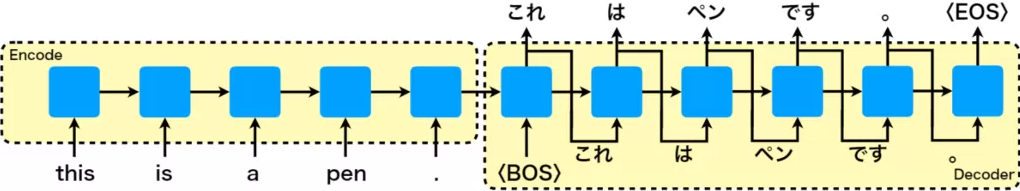
\includegraphics[scale=0.5]{seq2seq_model.png}
\caption{Seq2Seqの構造}
\label{seq2_model}
\end{figure}
\newpage
 しかし,Seq2Seqのデメリットは,入力系列のサイズに関わらず,固定長の特徴ベクトルに符号化されることである.これは,エンコーダのRNNの隠れ層で伝搬されてきた特徴ベクトルが,入力の長さに関係なく一定サイズでデコーダに渡されるため,入力系列が長い場合に前半の入力情報を覚えきれない.\\

\subsection{Seq2Seq with Attention}
 そこで次に提案されたのが,Seq2SeqにAttention機構を取り入れた\textbf{Seq2Seq with Attention}である.エンコーダの最後の潜在状態のみをデコーダで受け渡していたSeq2Seqに対して,Seq2Seq with Attentionでは,次の単語を予測するのに適する入力単語群へのアテンションを用いた\textbf{コンテキストベクトル}を導入しており,デコーダに対する入力を動的に変化させることができる.\\
 Seq2Seq with Attentionは,図\ref{seq_attention}のような構造をとっており,大きな手順は以下の通りである.\\

\hrule height 0.3mm depth 0.3mm width 140mm
\begin{enumerate}
\item モデル内のデータに対して,Attention機構を用いた処理を行う.\\
 通常のSeq2Seqモデルにおいて(エンコーダRNNの潜在ベクトル(隠れ層の系列)を$\{\mathbf{s}_1, \mathbf{s}_2 \cdots, \mathbf{s}_j, \cdots \mathbf{s}_N\}$,デコーダRNNの潜在ベクトルを$\{\mathbf{h}_1, \mathbf{h}_2, \cdots, \mathbf{h}_i, \cdots \mathbf{h}_M\}$とする),現ステップ$i$の潜在ベクトル$\mathbf{h}_i$から,$\mathbf{h}_{i+1}$を予測したい.\\
 このときのモデル内のデータの処理として,$\mathbf{h}_i$に対する,入力文書中の各単語の隠れ変数$\mathbf{s}_j(j\in\{1,2,\cdots ,N\})$の\textbf{アテンション係数}$a_i(j)$を,\textbf{スコア関数}を用いて予測する.
アテンション係数とは,以下の式で計算される.
\begin{equation}
a_i (j) = \frac{\exp(\rm{score}(\mathbf{s}_j, \mathbf{h}_i))}{\sum^N_{j'=1}\exp(\rm{score}(\mathbf{s}_j', \mathbf{h}_i))}
\end{equation}
 スコア関数$\rm{score}(\cdot)$は,$\mathbf{s}_j$,$\mathbf{h}_i$二つのベクトル間の関連度を示す単純な関数である.例として,$\mathbf{s}_j\cdot\mathbf{h}_i$(二つのベクトルの内積)や,$\mathbf{s}_j\cdot\mathbf{W}_a\mathbf{h}_i$などがある.これらは設計時に自由に決める.\\


\item コンテキストベクトル$\mathbf{c}_i$を計算する.\\
 コンテキストベクトルは以下の式で表される.
\begin{eqnarray}
&\mathbf{c}_i = \sum^N_{j=1} a_i(j)\mathbf{s}_j\\
                 &= a_i(1)\mathbf{s}_1+a_i(2)\mathbf{s}_2+\cdots+a_i(N)\mathbf{s}_N \nonumber  
\end{eqnarray}
 コンテキストベクトルは,翻訳後の単語が翻訳前の単語それぞれに対してどのくらい関連性があるのかの総和をとっている.\\

\item コンテキストベクトル$\mathbf{c}_i$を入力に加え,次のフレーム$i+1$を,デコーダで予測する.その後に潜在ベクトル$\mathbf{h}_{i+1}$から単語$\mathbf{y}_{i+1}$を予測する.\\

\item 上記の手順を,$<$EOS$>$が次の単語として予測されるまで繰り返す.

\end{enumerate}
\hrule height 0.3mm depth 0.3mm width 140mm
\vspace{5mm} 
 このSeq2Seq with Attentionの登場により,機械翻訳の精度がより高まったが,RNNによる逐次的なデータ処理によってデータの並列化が出来ないままであり,高速な処理を行うことが出来なかった.なので,並列計算を不可能にしていたRNNを取り除き,並列可能としたモデルとして,次節に示すTransformerが提案された.\\

\begin{figure}[H]
\centering
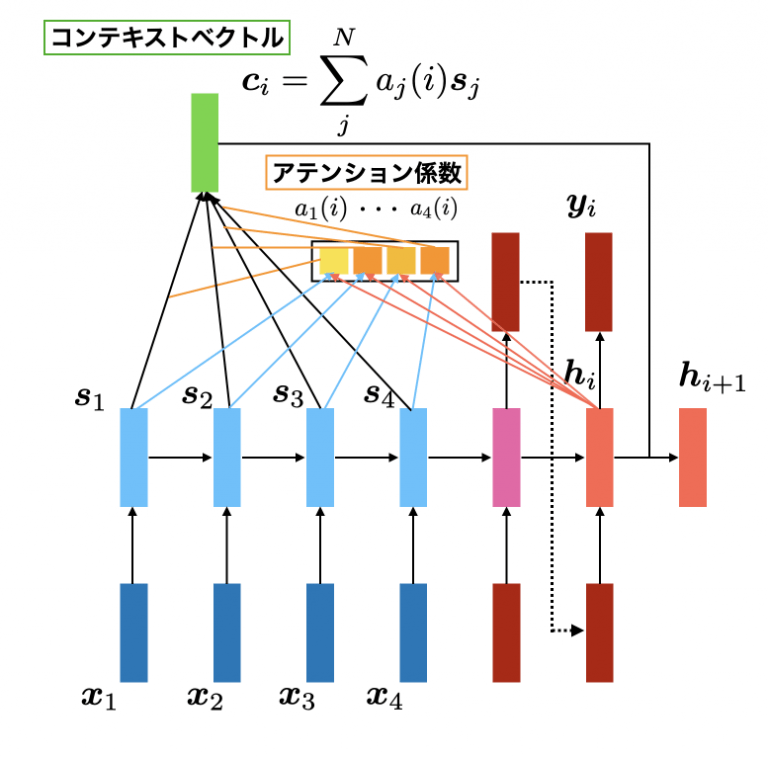
\includegraphics[width=9cm]{seq2seq_with_attention_model.png}
\caption{Seq2Seq with attentionの構造}
\label{seq_attention}
\end{figure}

\newpage
\section{Transformer}
 Transformerは図\ref{tra_model}のような構造をとっている.

\begin{figure}[H]
\centering
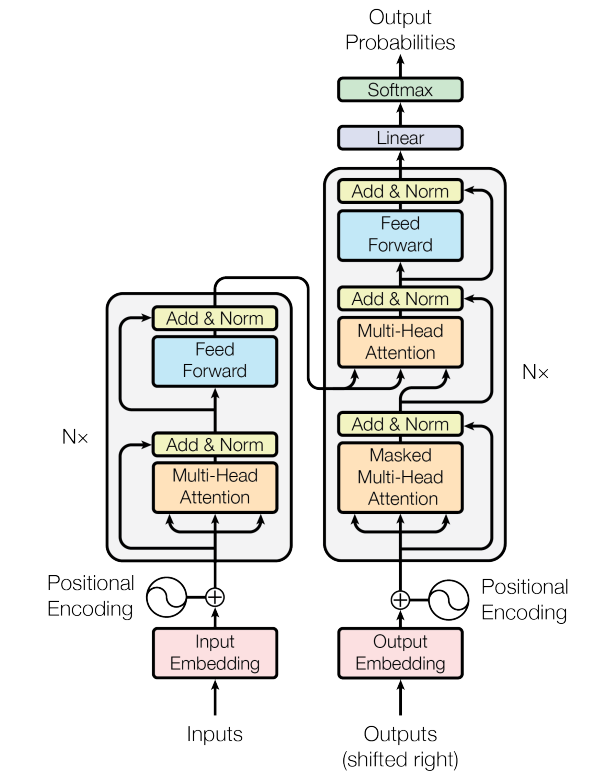
\includegraphics[width=8cm]{transformer_model.png}
\caption{Transformerの構造}
\label{tra_model}
\end{figure}

 図からもわかる通り,TransformerではRNNやCNNを一切使用せずにAttention機構のみで実装されている.これにより逐次的な処理を必要とせず,並列計算が可能となったため,GPUによる高速演算が可能となった.また,より長文の依存関係を掴むことができるようになった.\\
 次節以降では,Transformerの各層について説明していく.
\subsection{Embedding}
 埋め込みとも呼ばれる.自然言語処理分野の埋め込みは,解析したい単語をその単語の意味を表す固定長ベクトルに変換することである.Transformerでは,デフォルトで512次元のベクトルに変換する.\\
 埋め込みの代表的な手法として,\textbf{Word2Vec}というニューラルネットワークで構成されたモデルがある.
 
\subsection{Positinal Encoding}
 自然言語を取り扱う上で,語順の情報は必要不可欠である.従来の提案手法ではRNNを用いていたため,語順の情報が保たれた状態で逐次的に処理を行っていた.これに対しRNNのないTransformerでは,語順情報を入力に与える必要があったため,Positional Encodingで語順の情報をベクトル化し(デフォルトで512次元),これをEmbedding化された固定長ベクトルの各要素に足し合わせている.\\
 具体的な変換方法は以下の通りである.$t$をその単語が何番目に出現したのかを表す整数,変換後のベクトルを$\mathbf{p}_t$,$\mathbf{p}_t$の要素を$p_t^{(i)}$,$d$は全要素数(デフォルトで512)とする.\\

\begin{align}
p_t^{(i)} = 
\begin{cases}
\sin (\sigma_k\cdot t) , & (i = 2k)\\
\cos (\sigma_k\cdot t) , & (i = 2k+1).
\end{cases}
\end{align}
 ただし,
\begin{align}
\sigma_k = \frac{1}{10000^{2k/d}}.
\end{align}
 式からもわかる通り,$p_t^{(i)}$は$t$を時間,$\sigma_k$を角周波数とするsin波,cos波で表される.sinとcosが交互に要素として変換されるので,$\mathbf{p}_t$は以下のように表される.
\begin{equation}
\mathbf{p}_t=[\sin(\sigma_1\cdot t), \ \cos(\sigma_1\cdot t), \ \sin(\sigma_2\cdot t), \ \cos(\sigma_2\cdot t), \cdots, \sin(\sigma_{d/2}\cdot t),\ \cos(\sigma_{d/2}\cdot t)]^T
\end{equation}

\subsection{Multi-Head Attention}
 Multi-Head Attentionの構造を図\ref{att_model}(右)に示す.Multi-Head Attentionは\textbf{Scaled Dot-Product Attention}を幾層か重ね,出力を連結(Concat)したものであることがわかる.このScaled Dot-Product Attentionは\ref{att_model}(左)のようなモデルであり,$\mathbf{Q}$(Query), $\mathbf{K}$(Key),$\mathbf{V}$(Value)の3つの入力を持ち,1つの値(ベクトル)を算出する.\\
 ※ちなみに,これ以降に登場するベクトルは,元論文に合わせて\underline{列ベクトル}とする.
\begin{figure}[H]
\centering
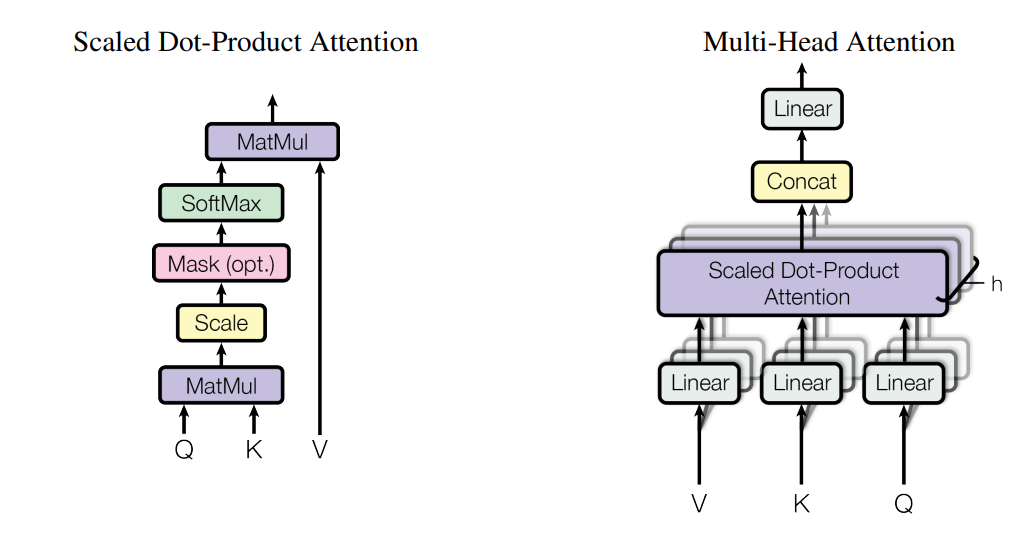
\includegraphics[width=8cm]{attentions.png}
\caption{Scaled Dot-Product AttentionとMulti-Head Attentionの構造}
\label{att_model}
\end{figure} 
 Scaled Dot-Product Attentionで用いられているAttention機構は以下の通りである.ここで,系列長(単語の数)を$ N$とすると,$\mathbf{Q}\in\mathbb{R}^{ N\times d_{q}}$,$\mathbf{K}\in\mathbb{R}^{ N\times d_{k} }$,$\mathbf{V}\in\mathbb{R}^{ N\times d_{v}}$である.ここで,$d_q = d_k$であり,元論文では強調されていないが,$d_v$も$d_k$と同じである.よって,入力の行列の列数は,すべて同じになる.\\
\begin{equation}
Attention(\mathbf{Q}, \mathbf{K}, \mathbf{V}) = softmax\left(\frac{\mathbf{Q}\mathbf{K}^T}{\sqrt{d_k}} \right)\mathbf{V}
\label{at_sca}
\end{equation}
 まず,QueryとKeyの内積(類似度)を計算し,$\sqrt{d_k}$で割ることによって,次元数$d_k$が大きい場合に内積が大きくなるのを防いでいる.それをソフトマックス関数に通し,最終的にValuesとの内積をとっている.したがって,最終的な出力は$\mathbb{R}^{ N\times d_{v}}$となる.\\

 このScaled Dot-Product Attention機構を組み合わせたMulti-Head Attentionは,以下の処理手順で計算される.\\
\hrule height 0.3mm depth 0.3mm width 140mm
\begin{enumerate}
\item 入力の$\mathbf{Q}, \mathbf{K}, \mathbf{V}$を構成する列ベクトル$\mathbf{x}$を,$d_{model}/h$の低次元ベクトルに射影する(デフォルトで$d_{modek}=512$,$h=8$).射影後の次元は$d_q = d_k = d_v = d_{model}/h = 512/8 = 64$となる.\\
 この射影を行うために,$i$番目($i\in\{1,  2, \cdots, h\}$)のヘッド個別の全結合層$\mathbf{W}_i^Q$,$\mathbf{W}_i^K$,$\mathbf{W}_i^V$との内積をとっている.\\
※ここで,入力$\mathbf{Q}, \mathbf{K}, \mathbf{V}$は,実はすべて同じ値である.これに対して固有の3種類の行列を掛けて射影することにより,抽出している特徴が異なっているが元の入力は同じの自己アテンション機構となっている.ここで,必ずしも入力は埋め込み層からではない.図\ref{tra_model}より,それぞれのエンコード,デコード機構はそれぞれ$N$回繰り返している.よって,最後のAdd\&Norm層からの入力であることもある.\\

\item 低次元に射影された$\mathbf{QW}_i^Q, \mathbf{KW}_i^K, \mathbf{VW}_i^V$を入力に,$h=8$個のScaled Dot-Product Attentionを実行する.よって,出力は8個の$\mathbf{Z}_1,\mathbf{Z}_2,\cdots, \mathbf{Z}_h$となる.\\

\item $\mathbf{Z}_i$の各出力を1つのベクトルに結合(Concatenation)する.よって,各列ベクトルの次元が$h\cdot d_v = 8\cdot 64 = 512$になる.\\

\item 結合したものを全結合層$\mathbf{W}^O$で変換する.$\mathbf{W}^O\in\mathbb{R}^{h\cdot d_v\times d_{model}}$であるため,最終的な次元は$d_{model}$となる.

\end{enumerate}
\hrule height 0.3mm depth 0.3mm width 140mm
\vspace{5mm} 
 数式で表すと以下のとおりである.\\
\begin{gather}
Multi-Head Attention(\mathbf{Q}, \mathbf{K}, \mathbf{V}) = Concat(\mathbf{Z}_1, \mathbf{Z}_2, \cdots, \mathbf{Z}_h)\mathbf{W}^o\\
\mathbf{Z}_i = Attention(\mathbf{QW}_i^Q, \mathbf{KW}_i^K, \mathbf{VW}_i^V)
\end{gather} 

\subsection{Feed Forward}
 Position-Wise Feed-Forward Networksとも呼ばれる.2層の全結合ニューラルネットワークであり,1層目の出力ではReLUに通し,2層目では値をそのまま出力(線形変換)している.このFF層をはさむことにより,Attention層で形成された位置情報込みの情報に対して,位置情報との依存関係を和らげ,一意なものとして変換することによって,表現力が増す(らしい).\\
 式を以下に示す.\\
\begin{equation}
\rm{FNN}(x) = \max (0, xW_1+b_1)W_2+b_2
\end{equation}

\subsection{Masked Multi-Head Attention}
 デコーダ側でも同様に,出力系列(翻訳したい言語)の埋め込みとPositional Encodingを行ったものを入力としているが,デコーダでは参照している単語の次の単語を予測する必要がある.エンコーダ側のMulti-Head Attentionでは入力した単語の系統のすべての情報を取りこんで類似度を学習しているため,次の単語の情報を必然的に参照している.そのため,未来の単語を参照できなくするために,未来の単語が入力されていた場所には別の入力を入れることでその情報を無効にしている.なので,入力が異なるだけで構造自体はエンコーダ側のMulti-Head Attentionと同じである.\\
 例えば,英語から日本語に翻訳したいとき,図\ref{seq2_model}の例をとると,以下のような入力が用意される.\\

  エンコーダ側:[This, is, a, pen, .]\\
  デコーダ側 :[\textless BOS 	\textgreater,これ, は, ペン, です, 。]\\
  
   最初のBOSとは,Beginning of Sentenceの略で文頭を表す仮想単語である.\\
  デコーダ側の入力は,まずBOSから入力して,他のデータはマスクされているのでBOSのみで学習を行い,出力で次の単語(この場合は「これ」)が出力されるように学習を行っていく.そして,次の単語が出力されたらその単語を新たな入力として,マスクを解除してあげることでまた次の単語を学習していく.\\
  
 ここで,別の入力とは,式(\ref{at_sca})のソフトマックス関数に対して$-\infty$を入力することである.$softmax_i= e^{x_i}/\sum_j e^{x_j}$なので,消したい$x_j$が$-\infty$になると,$e^{x_j} \rightarrow e^{-\infty}=0$となるからである.\\

\subsection{デコーダでのMulti-Head Attention}
 デコーダではMusked Multi-Head Attentionのあとにもう一つMulti-Head Attentionを設けている.このMulti-Head Attentionの入力は,入力系列をエンコーダに通したあとの値を$\mathbf{X}$,出力系列をMasked Multi-Head Attentionに通したあとの値を$\mathbf{Y}$とすると,$\mathbf{Q}=\mathbf{Y},\mathbf{K}=\mathbf{X},\mathbf{V}=\mathbf{X}$としている.すなわち,\uline{翻訳後(Query)の単語}が\uline{翻訳前(Key-Value)のどの部分に注目するか}を学習することができる.\\
 このように,2系列間で各トークン表現間の関連度を計算するAttention機構を,\textbf{Source-Target Attention}という.対して,今まで紹介してきたMulti-Head Attentionは,1つの系列内での各トークン表現間の関連度を計算するAttention機構であり,これを\textbf{Self Attention}と呼ぶ.\\

\subsection{その他の機構}
\begin{itemize}
\item \textbf{残差接続}\\
 Transformerでは,5種類の層で残差接続を行っている.\\
 残差接続とは,図\ref{re}に示すような接続であり,入力の値を出力の値に足し合わせて活性化を行う機構である.残差接続を行うことにより勾配消失問題などを解決できるため,Transformerはより多くの層を増やすことが可能となった.
\begin{figure}[H]
\centering
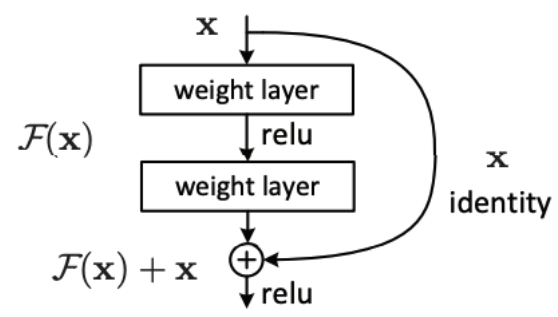
\includegraphics[width=8cm]{residual.png}
\caption{残差接続の構造}
\label{re}
\end{figure} 


\item \textbf{レイヤー正規化}\\
 層の出力に対して平均を0,分散1に正規化する手法である.バッチ正規化では一つひとつの別々の値の対応する要素に対して正規化を行っているが,レイヤー正規化では,一つの値の要素に対して正規化を行っている.\\
 式で表すと以下のようになる.ここで,$h(t,i)$はt番目の単語のi番目の要素を表しており,$\gamma, \beta$は学習可能なパラメータである.
\begin{align}
\mu(t) &= \frac{1}{d_{model}}\sum_{i=1}^{d_{model}}h(t,i)\\
\sigma(t) &= \sqrt{\frac{1}{d_{model}}\sum_{i=1}^{d_{model}}(h(t,i)-\mu(t))^2}\\
LayerNorm(h, t) &= \frac{\gamma}{\sigma(t)}\odot(h(t,i)-\mu(t))+\beta
\end{align}
\vspace{10mm}


 よって,最終的に,Add\&Normは次のように表記できる.
\begin{equation}
 ResidualLayerNorm(x) = LayerNorm(sub_block(x)+x)
\end{equation}
\end{itemize} 

\section{まとめ}
 本ゼミでは,自然言語処理のエンコーダ・デコーダモデルから,Transformerの構造について説明を行った.Transformerは近年のNLPで主力となっているBERTやXLNet,GPTなどのベースとなっているため,学習していて,自然言語処理の歴史について学習することが出来た.実装まで至らなかったので,次のゼミでは何かしらの実装を行って発表したい.
 


\begin{thebibliography}{99}
\bibitem{all}Vaswani, Ashish, et al. "Attention is all you need." Advances in neural information processing systems 30 (2017). 
\end{thebibliography}
\end{document}
